\section{Image Generation}

\subsection{Overview}

Training images are vital to our task. Computer generated images are too standard to contain enough noise, making our model vulnerable to possible noisy test images; hand-drawn sketches are too noisy, on the other hand, raising challenges for image feature extraction and complicating our rules. Both senarios could diminish the generalization ability of our model. Therefore we use the following three different kinds of images:

First in the system prototyping stage, we use a painting tool to draw several images of \textbf{circles, ellipses, triangles, rectangles and squares} as the \textbf{prototyping set}. Note that these images are not generated in vector format on purpose, thus introducing small noises at a pixel level. We hope that by analyzing these quasi-standard images, we can derive the basic framework of our system.

Then we use image processing techniques to distort and rotate the standard figures, obtaining a great amount of images and split them into \textbf{training set, developing set and testing set}. Now we can use the training set to determine the fuzzy sets and the developing set to tune the fuzzy sets and rules based on error analysis.

Finally in the testing stage, we use the testing set to evaluate our system. We also ask different people to \textbf{draw sketches with a digitized tablet} for measuring performance. We decide not to use mouse because that would produce overly noisy images.

Note that for the convenience of development, \textbf{all images we use only contain one shape except for the sketch images}. In other words the final system is intended to perform well with sketches containing multiple (non-overlapping) figures.

\subsection{Details}

\subsubsection{Computer-generated Images}

Images are generated as follows:

First we generate a random image of the target shape. Then we \textbf{distort the contour} of the figure by applying a Sine function on each row and column of the image, with a given factor to control the distorting effect. At last image is \textbf{rotated} by a random angle.

Finally we obtain 2000 images for each shape, and we split them into \textbf{training set}, \textbf{developing set} and \textbf{testing set} with a $8:1:1$ ratio.  The images look like this. (Figure 1)

\begin{figure}[ht!]
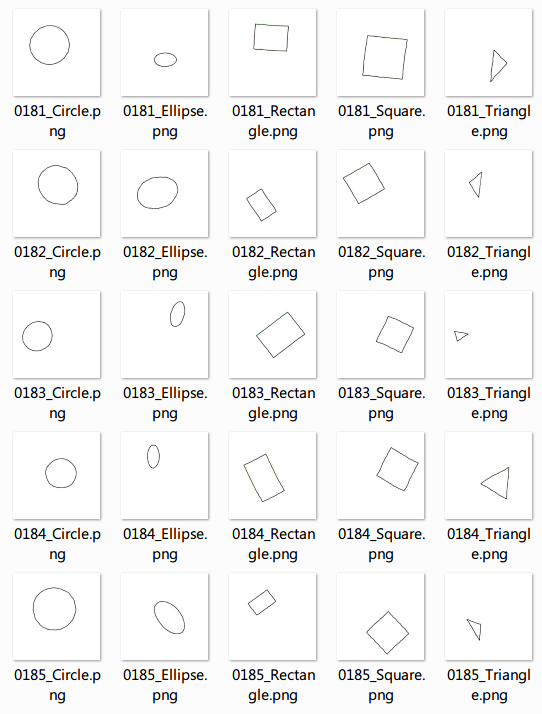
\includegraphics[width=\columnwidth]{Figure_1_CG_Image.png}
\caption{Computer-generated Images}
\end{figure}

\subsubsection{Hand-drawn Sketches}

The sketches are drawn by two difference people. They look like this. (Figure 2)

\begin{figure}[ht!]
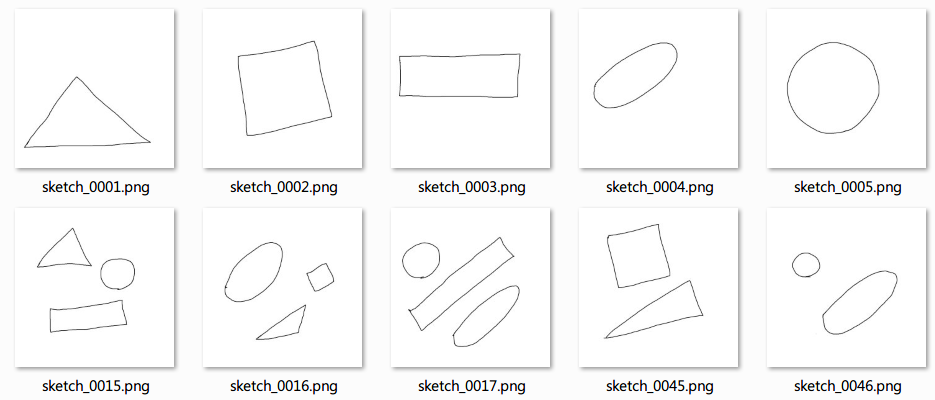
\includegraphics[width=\columnwidth]{Figure_2_Sketch_Image.png}
\caption{Hand-drawn Sketches}
\end{figure}
